\chapter{Описание моделей, отвечающих за генерацию поведения виртуального актора}


В данном разделе приводится теоретическое описание модели.

\section{Постановка задачи}

В рамках научно-исследовательской работы был расширен подход решения поставленной задачи задачи, который выражается в
использовании машинного обчучения. Данный подход используется в совокупности когнитивной архитектурой eBICA. 
eBICA – “emotional biologically inspired cognitive architecture” – “эмоциональная биологически вдохновленная когнитивная архитектура”. 

В этой архитектуре эмоциональные элементы добавлены практически ко всем процессам за счет модификации основных строительных блоков архитектуры. 
Ключевым моментом этой когнитивной архитектуры являются оценки, которые связаны со схемами и психическими состояниями как их атрибуты, 
моральные схемы, которые контролируют модели оценок и представляют социальные эмоции, а также семантические пространства, которые дают 
значения этих оценок.

Как видно из (Рис. \ref{pic:ris7}), архитектура представляет собой конгломерат компонентов: интерфейсный буфер, рабочая, процедурная, семантическая 
и эпизодическая системы памяти, система ценностей и система когнитивных карт \cite{Samsonovich01}. Три основных строительных блока для этих компонентов - это 
ментальные состояния, схемы и семантические карты. Семантическая память - это коллекция определений схем. Буфер интерфейса заполняется схемами.

\begin{figure}[h]
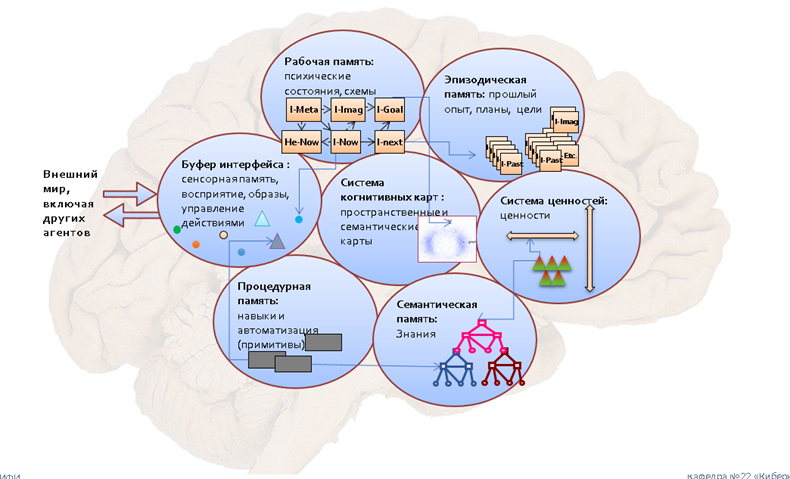
\includegraphics[width=0.75\columnwidth]{./img/ris7.png}
\centering  
\caption{Структура когнитивной архитектуры eBICA}
\label{pic:ris7}
\end{figure}

Рабочая память включает активные психические состояния. Эпизодическая память хранит неактивные психические состояния, сгруппированные 
в эпизоды - предыдущее содержимое рабочей памяти. Следовательно, эпизодическая память состоит из структур, аналогичных тем, которые 
обнаруживаются в рабочей памяти, но которые «заморожены» в долговременной памяти. Процедурная память включает в себя примитивы. Система 
ценностей включает в себя шкалы, представляющие основные значения. Система когнитивных карт включает, в частности, семантические карты 
эмоциональных ценностей. Семантическая карта использует абстрактное метрическое пространство (семантическое пространство) для представления 
семантических отношений между ментальными состояниями, схемами и их экземплярами, а также для присвоения значений их оценкам.


\section{Описание работы модели актора}

На момент начала выполнения работы уже была реализована система работы виртуальных агентов, и она состоит в том, что сперва 
считываются действия и объекты с заданными для них параметрами и значениями из Excel файла, а также инициализируются значения. 
Затем выбор действий происходит в следующем порядке: в радиусе вокруг оценок виртуального актора выбираются действия, которые 
попадают в этот радиус, а также проверяются различные условия, необходимые для выполнения действия. Если условия не выполняются, 
то действие не может быть выбрано. Затем, после того как в список добавлены все действия, которые могут быть выполнены, рассчитываются 
вероятности на основе оценок и рассчитанных констант. Также, если действие повторное, его вероятность несколько занижается. 
После расчета вероятностей выбирается действие, которое влияет на оценки виртуального актора. 

Помимо этого происходит замена состояний объектов и виртуальных акторов. После этого происходит перерасчет оценок Appraisals и Feelings \cite{Samsonovich01}.

Основная модель eBICA определяет поведение виртуального актора исходя из следующих факторов:

\begin{itemize}
  \item соматический;
  \item рациональный;
  \item когнитивный.
\end{itemize}

Нравственный фактор регулирует отношения первого актора со вторым на основе системы ценностей (представленной семантической картой) 
и моральных схем. Под когнитивным фактором понимается учет соображений нравственности, этики и морали, общей системы ценностей, 
понятий о добре и зле, о собственном достоинстве, эмпатии, соображений эстетики, стремлений к простоте и элегантности, и т.д. 
Учет этих соображений возможен на основе когнитивных оценок (appraisals) всех релевантных агентов, событий, их возможных действий 
и последствий этих действий, фактов, свойств, отношений, и т.д. Возможен вариант модели, в которой ответное действие может выбираться 
лишь из двух вариантов: положительная реакция на действие человека и отрицательная. Данная версия модели весьма неплохо работает даже 
с таким ограничением. Но невозможно придерживаться данной парадигмы при увеличении количества возможных вариантов для взаимодействия 
между акторами. В данной модели необходимо учесть пересчет оценок Appraisals и Feelings. Для пересчета оценок Appraisals используется 
следующая формула \ref{eq:appraisals01}:

\begin{equation}
  \begin{gathered}
    Appraisals=(1-r)*Appraisals+r*Action
    %P_{i+1j  } (R_{i+1j  } , {\varphi}_{i+1} , {\theta}_{j  }) \\
  \end{gathered}
  \label{eq:appraisals01}
\end{equation}

где Appraisals - оценка, 
r - эмпирически вычисленная константа экспоненциального затухания, 
Action - оценка совершаемого действия на семантической карте.

Одновременно с Appraisals пересчитываются так называемые “чувства” Feelings согласно режиму работы моральной схемы.
Аффективное пространство VAD – это трехмерное векторное пространство, точки которого соответствуют определенным эмоциональным 
состояниям, или аффектам, представленным триплетами значений (Valence, Arousal, Dominance). 
Существуют и сходные модели: PAD (Pleasure, Arousal, Dominance), EPA (Evaluation, Potency, Arousal) и другие. 
Здесь мы используем модель VAD. Соответственно, под «семантической картой» здесь часто понимается ее конкретная 
разновидность: аффективная карта (или когнитивная семантическая карта).

Шкалы имеют следующие значения:
\begin{itemize}
  \item dominance – варьируется при значении от 0 (покорность) до +1 (доминантность) и описывает соответствующие чувства; 
  \item valense – при значениях от -1 до 0 показывает уровень негатива или радости соответственно; 
  \item arousal – значения от -1 до 1 показывают уровень возбуждения (заинтересованности), к примеру, гнев по уровню возбуждения сильнее раздражительности, но слабее ярости. 
\end{itemize}

Оценки представлены в виде векторов на трехмерной семантической карте \cite{seman_karta}, \ref{pic:ris5}.
Моральная схема определяет общую установку на оценку поведения акторов, согласно их ролям и типу ситуации. 
Ее целью (как агента) является достижение и поддержание «нормального» положения дел, определенного набором Feelings. 
Вообще говоря, моральная схема состоит из двух частей: части, распознающей тип ситуации и осуществляющей привязку (binding),
и части, реализующей динамику схемы. В случае парадигмы актора можно считать, что моральная схема одна, уже привязана, и 
потому первая часть ее не актуальна.

Субъективные оценки (Feelings) генерируются по определенным правилам на основании истории объективных оценок и состояний системы. 
Грубо говоря, Feelings – это субъективное представление о том, каким оцениваемый актор является «на самом деле», и, следовательно, 
какого поведения от него нужно ожидать и на какое место его нужно ставить своим поведением. Следовательно, выбор поведения актора 
должен осуществляться так, чтобы приблизить Appraisals к Feelings. 

Значение Feelings определяет моральная схема, которая может работать в одном из трех режимов. 
Первый режим основывается на формуле \ref{eq:feelings01}:

\begin{equation}
  \begin{gathered}
    Feelings=beta*Appraisals
  \end{gathered}
  \label{eq:feelings01}
\end{equation}

где beta – эмпирически вычисленная константа. 

В данном режиме схема говорит, что если актор ведет себя хорошо, то к нему нужно относиться как к хорошему, и т.д. 

Цель данного процесса – распознать и классифицировать актора, выработать отношение к нему и приписать ему определенную роль во взаимоотношениях. 

В данном режиме моральная схема работает пока разница между квадратами норм Feeling и Appraisals не станет меньше некоторого значения.

Суть второго режима заключается в том, что значение Feeling фиксировано и экстремально по абсолютной величине, т.е. находится на сфере, 
ограничивающей семантическую карту (предположим, что есть такая сфера). Направленность вектора Feeling может быть либо произвольной, 
определенной предысторией, либо дискретной – вдоль одной из осей.

Третий режим состоит в том, что значения Feelings меняются \ref{eq:feelings02}, подстраиваясь под текущие значения Appraisals (здесь r1 может быть отличным от r): 

\begin{equation}
  \begin{gathered}
    Feelings=(1-r_1 )*Feelings+r1*(Appraisal-Feelings)
  \end{gathered}
  \label{eq:feelings02}
\end{equation}

Соответственно значения Appraisals и Feelings как говорится в работе \cite{Samsonovich05} пересчитываются после каждого действия первого актора, направленного на второго актора.
Также пересчет оценок происходит после определения и совершения одним из акторов ответного или самостоятельного действия. 
В данном контексте под термином “самостоятельное действие” имеется в виду действие, основанное лишь на текущем состоянии мира и 
значений векторов Appraisals и Feelings акторов, отобрежнные на (Рис. \ref{pic:ris8}). 


\begin{figure}[h]
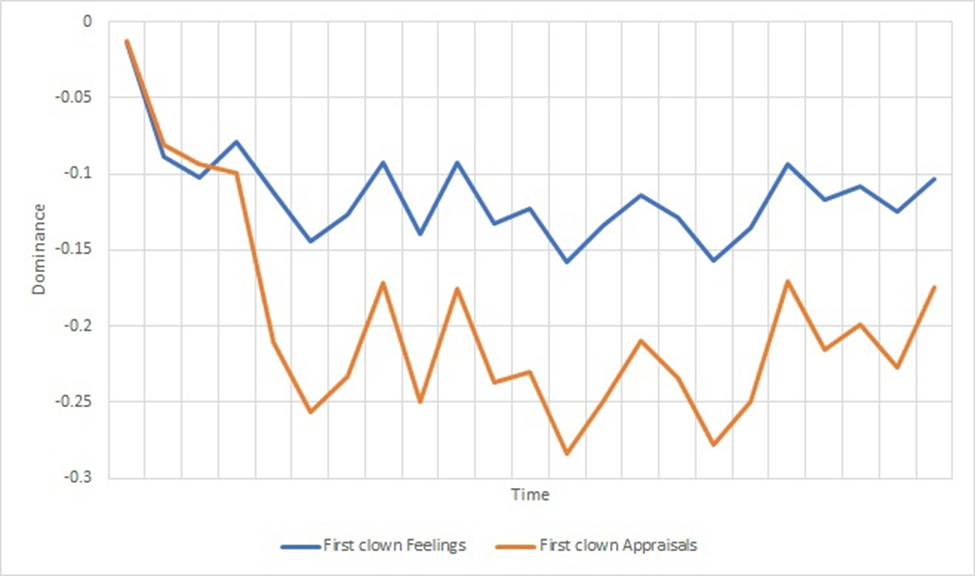
\includegraphics[width=0.75\columnwidth]{./img/ris8.png}
\centering
\caption{Корреляция значений Appraisals (оранжевая) и Feelings (синяя) для показателя доминантности на протяжении времени/действий с шагом в 5 секунд}
\label{pic:ris8}
\end{figure}

Согласно (Рис. \ref{pic:ris8}) мы видим, что работа модели сводится к выбору действия, 
которое будет максимально приближать Appraisals к Feelings и вектор соматического состояния к начальному положению.

\section{Распознавание речи}

Как было упомянуто ранее, для распознавания речи используются акустические модели, однако этого 
может быть недосточно, так как словари на текущий момент состоят из 
миллионов, а то и триллионов слов, многие из них совпадают по своему звучанию и могут даже совпадать и в написании и в зучании.

За основной параметр в использовании распозвавания речи при испоьзовании классической акустической модели - 
берется фонема, однако в слове она может находиться в трех раличных состояниях: начало, середина и конец.
фонемы являются позиционно-зависимыми и контекстно-зависимыми: формально «одна и та же» фонема звучит существенно по-разному в зависимости от того, 
в какой части слова она находится и с какими фонемами соседствует. Вместе с тем, простое перечисление всех возможных вариантов контекстно-зависимых фонем 
вернет очень большое число сочетаний, многие из которых никогда не встречаются в реальной жизни; чтобы сделать количество рассматриваемых акустических событий разумным, 
близкие контекстно-зависимые фонемы объединяются на ранних этапах тренировки и рассматриваются вместе.

Тренировка акустической модели — сложный и многоэтапный процесс. Для тренировки используются алгоритмы семейства Expectation-Maximization, такие, как алгоритм Баума-Велша. 
Суть алгоритмов такого рода — в чередовании двух шагов: на шаге Expectation имеющаяся модель используется для вычисления матожидания функции правдоподобия, 
на шаге Maximization параметры модели изменяются таким образом, чтобы максимизировать эту оценку 
(Рис. \ref{pic:expectmax}). 

\begin{figure}[h]
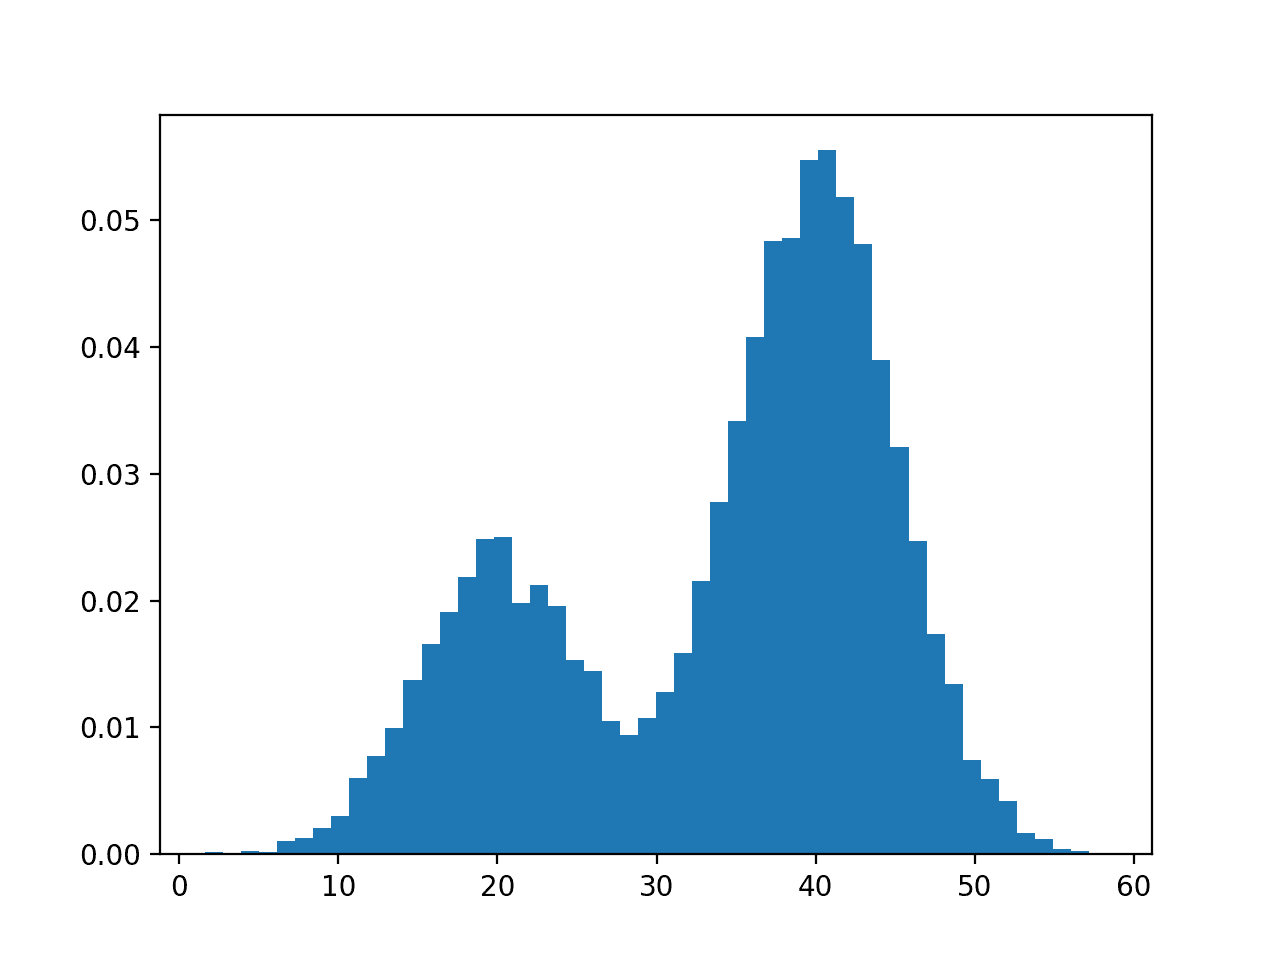
\includegraphics[width=0.75\columnwidth]{./img/expect_max.png}
\centering
\caption{Гистограмма набора данных, построенная из двух разных гауссовских процессов}
\label{pic:expectmax}
\end{figure}

На ранних этапах тренировки используются простые акустические 
модели: на вход даются простые MFCC features
(Рис. \ref{pic:mel}), фонемы рассматриваются вне контекстной зависимости, для моделирования вероятности эмиссии в HMM используется смесь 
гауссиан с диагональными матрицами ковариаций (Diagonal GMMs — Gaussian Mixture Models).

\begin{figure}[h]
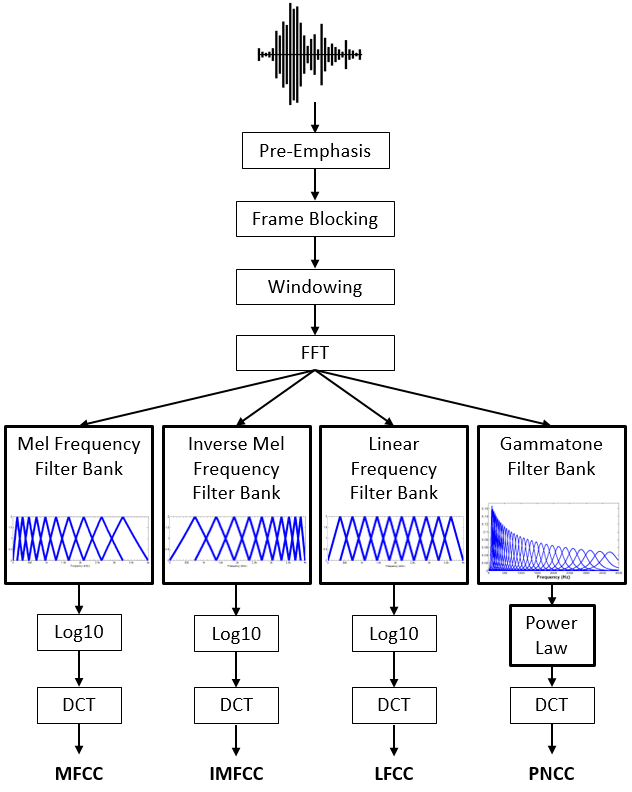
\includegraphics[width=0.75\columnwidth]{./img/mel.png}
\centering
\caption{Четыре метода выделения признаков MFCC, IMFCC, LFCC и PNCC}
\label{pic:mel}
\end{figure}
  

Результаты каждой предыдущей акустической модели являются 
стартовой точкой для тренировки более сложной модели, с более сложным входом, выходом или функцией распределения вероятности эмиссии. 
Существует множество способов улучшения акустической модели, однако наиболее значительный эффект имеет переход от GMM-модели к DNN (Deep Neural Network), 
что повышает качество распознавания практически в два раза. Нейронные сети лишены многих ограничений, характерных для гауссовых смесей, и обладают лучшей обобщающей способностью. 
Кроме того, акустические модели на нейронных сетях более устойчивы к шуму и обладают лучшим быстродействием.


Нейронная сеть для акустического моделирования тренируется в несколько этапов. Для инициализации нейросети используется стек из ограниченных машин Больцмана 
(Restricted Boltzmann Machines, RBM). RBM — это стохастическая нейросеть, которая тренируется без учителя. Хотя выученные ей веса нельзя напрямую использовать 
для различения между классами акустических событий, они детально отражают структуру речи. Можно относиться к RBM как к механизму извлечения признаков (
feature extractor) — полученная генеративная модель оказывается отличной стартовой точкой для построения дискриминативной модели. 
Дискриминативная модель тренируется с использованием классического алгоритма обратного распространения ошибки, при этом применяется ряд технических приемов, 
улучшающих сходимость и предотвращающих переобучение (overfitting). В итоге на входе нейросети — несколько фреймов MFCC-features 
(центральный фрейм подлежит классификации, остальные образуют контекст), на выходе — около 4000 нейронов, соответствующих различным сенонам. 
Эта нейросеть используется как акустическая модель в production-системе.

\section{Рекуррентные нейронные сети}

LSTM — это класс возвратных нейронных сетей. Поэтому, прежде чем мы сможем перейти к LSTM, 
важно понять нейронные сети и рекуррентные нейронные сети \cite{Wikipedia01}. 

Нейронные сети - Искусственная нейронная сеть представляет собой слоистую структуру из связанных нейронов,
вдохновленную биологическими нейронными сетями. Это не один алгоритм, а комбинация различных алгоритмов, 
которая позволяет нам выполнять сложные операции с данными. 
Рекуррентные нейронные сети - это класс нейронных сетей, предназначенных для работы с временными данными. 
Нейроны RNN имеют состояние / память ячейки, и ввод обрабатывается в соответствии 
с этим внутренним состоянием, которое достигается с помощью петель в нейронной сети. 
В RNN существуют повторяющиеся модули «tanh» слоев, которые позволяют им сохранять информацию. 
Однако ненадолго, поэтому нам нужны модели LSTM. 

LSTM - Это особый вид рекуррентной нейронной сети, способной изучать долгосрочные зависимости в данных. 
Это достигается за счет того, что повторяющийся модуль модели имеет комбинацию четырех слоев, взаимодействующих друг с другом \cite{Wikipedia01}. 

На (Рис. \ref{pic:ris9}) отображены структуры вышеупомянутые виды рекуррентных сетей: 

\begin{figure}[h]
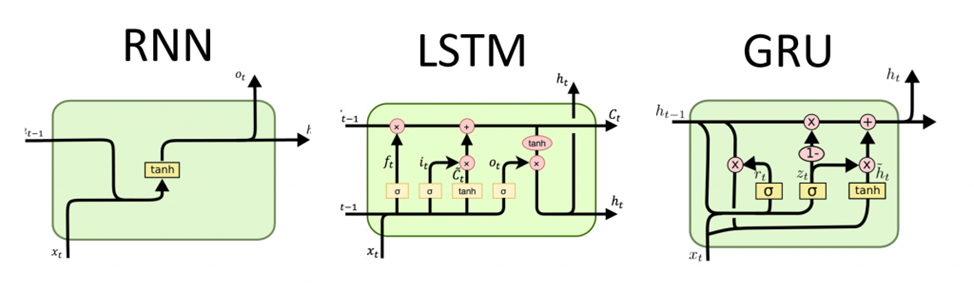
\includegraphics[width=0.75\columnwidth]{./img/ris9.png}
\centering
\caption{Структуры рекуррентных нейронных сетей}
\label{pic:ris9}
\end{figure}

\section{Выводы}

% В данном разделе была сформулирована постановка задачи, рассмотрены возможные ее решения с помощью архитектуры eBICA и подхода с использованием машинного обучения. 
% Выделен подход для распозвавания речи.

Было изучено описание работы модели виртуального актора. Изучены подходы и методы применительно к задаче распознавания речи.
Были рассмотрены ключевые подходы машинного обучения, которые будут использоваться в работе, а именно рекуррентные нейронные сети
